\documentclass[11pt]{article}

\usepackage{titlesec}
\usepackage{graphicx}
\usepackage{caption}
\usepackage{subcaption}
\usepackage{amsmath}
\usepackage{amsfonts}
\usepackage{amssymb}
\usepackage{hyperref}
\usepackage{enumitem}
\usepackage{listings}
\usepackage{xcolor}

% Define colors for syntax highlighting
\definecolor{mygreen}{rgb}{0,0.6,0}
\definecolor{mygray}{rgb}{0.5,0.5,0.5}
\definecolor{mymauve}{rgb}{0.58,0,0.82}

% Set up the MATLAB code listing style
\lstset{
  backgroundcolor=\color{white},
  basicstyle=\footnotesize\ttfamily,
  breakatwhitespace=false,
  breaklines=true,
  captionpos=b,
  commentstyle=\color{mygreen},
  deletekeywords={...},
  escapeinside={\%*}{*)},
  extendedchars=true,
  frame=single,
  keepspaces=true,
  keywordstyle=\color{blue},
  language=Matlab,
  otherkeywords={*,...},
  numbers=left,
  numbersep=5pt,
  numberstyle=\tiny\color{mygray},
  rulecolor=\color{black},
  showspaces=false,
  showstringspaces=false,
  showtabs=false,
  stepnumber=1,
  stringstyle=\color{mymauve},
  tabsize=2,
  title=\lstname
}


% Adjust the margins if needed
\usepackage[left=1in, right=1in, top=1in, bottom=1in]{geometry}
\usepackage{graphicx}
\usepackage{graphicx}
\usepackage{tabto}

% Set the title and author
\title{Newton's Method, Error, Newton's Fractal and Explorations}
\author{David Tran and Spencer Kelly}
\date{\today}

\begin{document}

\maketitle

\subsection*{Abstract}

In the following, we explore and provide an implementation of Newton's method for both simple roots and roots of multiple multiplicity. We discuss how to determine the order of convergence, as well as how to approximate the order of convergence for functions whose roots are unknown. Also, due to differences in convergence for roots of multiple multiplicity, we show a modified version of Newton's method which can speed up convergence up to the expected quadratic speed for multiplicity $m > 1$. In the final sections, we show how Newton's method can be used to generate Newton's fractals, and generate fractals for the fourth roots of unity and the Mandelbrot set.

\section{Introduction}

(See References section for references used here.)

This is the second lab in a series of 4 labs exploring various numerical algorithms and analyzing their properties. Finding roots of polynomials has been a significant area of interest throughout the entirety of the history of mathematics. As evidence to this claim, consider the fact that entire branches of mathematics were born out of the desire to find roots of polynomials. For example, group theory takes its roots from Galois' proof of the insolvability of the quintic.

In this lab, we discuss Newton's method, an algorithm discovered by Issac Newton and Joseph Raphson. The algorithm comes from a family of iterative root-finding algorithms: algorithms which generate successively better approximations of the root of a function. Another type of root-finding algorithms are bracketing methods, which successively narrow the range in which a root may be found until a desired precision. However, many of these methods, such as the bisection method, converges much slower than Newton's method (e.g., only a single extra bit of precision for each iteration in the case of the bisection method), so algorithms such as Newton's method are often used in practice.

Newton's method is especially important due to the prevalance of the problem of finding roots in numerous applications. In particular, it is useful for when only an approximate solution to an equation is needed, especially when the exact solution would require far more computational power. For example, consider the problem of rendering the shadows of certain voxels in the context of computer graphics. To the naked eye (and more importantly, the resolution of the screen), only a finite amount of precision is needed to calculate the reflection and physics of light for a realistic image. Thus, we see Newton's method effectively being used to calculate raytracing and pixel shadowing for millions, sometimes billions, of voxels, which would otherwise be computationally intractable if we desired exact solutions.


\section{Newton's Method}

\subsection{Implementation}

Newton's method is a fixed-point iteration method used to approximate the roots of a real-valued function. We implement a method that returns the iterates
% in Figure~\ref{fig:mynewton.m}.
\lstinputlisting{mynewton.m}
\subsection{Testing}

We test the method with the function:

$$
f(x) = (x + 1)(x - 1/2)
$$
for which we expect the roots $x = -1$ and $x = 1/2$. The derivative is
$$
f'(x) = 2x + 1/2
$$
so we test with the code below which returns the iterates as follows
% in Figure~\ref{fig:test_mynewton.m}
\lstinputlisting{test_mynewton.m}
\begin{align*}
x1 &= [-1.2000, -1.0211, -1.0003, -1.000] \\
x2 &= [0.6000, 0.5059, 0.5000, 0.5000]
\end{align*}
which we see properly approaches $-1$ and $0.5$.

\subsection{Determining Order of Convergence}

We use the code in Figure~\ref{fig:newtontest.m} to plot the logarithms of the errors against each other for $x = -1$ in Figure~\ref{fig:newton_root_1} and $x = 1/2$ in Figure~\ref{fig:newton_root_2}.

$$
\log_e \vert e_{k + 1} \vert \approx \alpha \log_e \vert e_k \vert + \log_e (C)
$$

Estimating a line-of-best-fit for both plots as seen in Figure~\ref{fig:newton_root_1_fit} and Figure~\ref{fig:newton_root_2_fit} shows an approximate slope $\alpha = 2$, corresponding to a quadratic order of convergence.

This matches the expected value of 2 that we should observe for Newton's method, since we expect it to have quadratic convergence. We expect this since Newton's method approximates the next iteration $x_{n + 1}$ with the solution to

$$
0 \approx f(x_{n + 1}) \approx f(x_n) + f'(x_n)(x_{n + 1} - x_n)
$$

which, solving for  $x_{n + 1} - x_n$ and taking the error at iteration $n$ as $e_n = r - x_n$ (where $r$ is the root), gives

$$
e_{n + 1} \approx -\frac{f(r - e_n)}{f'(r - e_n)}
$$

and thus Taylor-expanding the right-hand side demonstrates a quadratic relationship between $e_{n + 1}$ and $e_n$ for some constant $C$ dependent on the second derivative of $f$:

$$  
e_{n + 1} \approx Ce_n^2.
$$

\subsection{Approximating Order of Convergence}

Determining the order of convergence is only possible when we know in advance the exact roots. However, often this is not the case. To detect quadratic convergence using only the information provided from our iterative approximates, we can compute the ratios of consecutives differences between iterates $x_n$ and $x_{n + 1}$. If the ratios are constant, then we are most likely observing quadratic convergence. This is a result of the fact that the second derivative of a quadratic function is constant.

We use the code in Figure~\ref{fig:estimateconvergence.m} to demonstrate the ratios for quadratic convergence of the original function of interest $f(x) = (x + 1)(x - 1/2)$ in Figure~\ref{fig:estimate_convergence}. We use an initial guess far from the true value, $x_0 = -1000$ to show that the ratios are constant as we converge. Notice how the ratios are constant around $0.5$ (they fall rapidly towards 0 as we approach the exact root of $-1$.)

If instead our root has multiplicity greater than 1, quadratic convergence is not guaranteed, and the method will most likely converge slower. To detect when converging to a multiple root one can observe the convergence and see if convergence is linear, or even slower. To approximately determine the multiplicity $m$ of such a root, one can use the fact that a root of multiplicity $m$ converges $m$ times slower than a simple root. Thus, a root of multiplicity $2$ converges linearly, a root of multiplicity $3$ converges sublinearly (square-root), etc. So, we can observe the higher-order ratios, and observe when their behaviour (either quadratic, linear, sublinear, etc.), to approximately determine the multiplicity.

If the multiplciity is known, say $m$, we can modify Newton's method as the following to converge to the multiple root with quadratic convergence:

$$
x_{n + 1} = x_n - m\left(\frac{f(x_n)}{f'(x_n)}\right)
$$

See the implementation in Figure~\ref{fig:modifiednewton} which results in the following convergence for a $f(x) = (x - 2)^3$, a function with root of multiplicity 3.

\begin{center}
  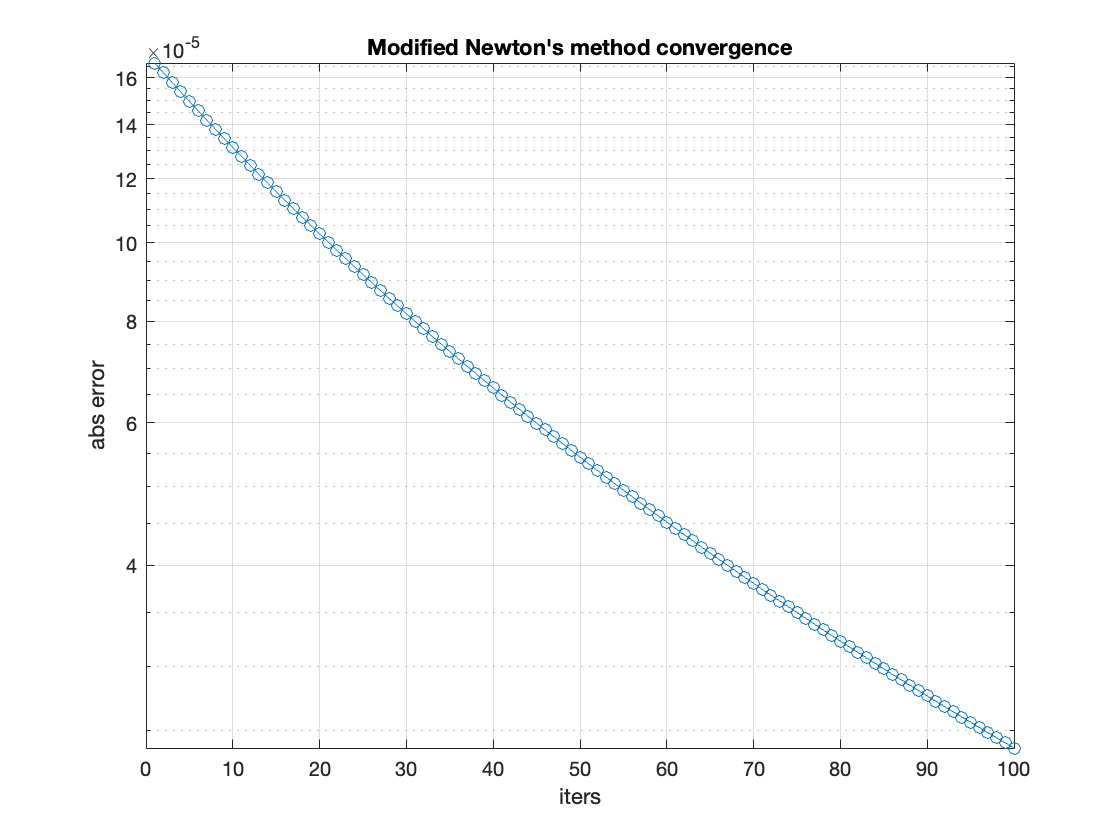
\includegraphics[width=0.7\linewidth]{modifiednewton.png}
\end{center}

\section{Newton's Fractals}

\subsection{Fourth Roots of Unity}

The solutions to $z^4 = 1$ can be solved using Euler's formula: since $\exp(i\theta) = \cos\theta + i \sin \theta$, $z^4 = 1$ is equivalent to $z^4 = \exp(i2\pi n)$ with $n$ an integer. Taking the fourth root gives $z = \exp(i2\pi n/4)$, which for $n = 0, 1, 2, 3$ yields the roots
\begin{align*}
  r_1 &= 1 \\
  r_2 &= i \\
  r_3 &= -1 \\
  r_4 &= -i
\end{align*}
and can be graphed on the complex plane by the red, green, orange, and pink lines, respectively below.

\begin{center}
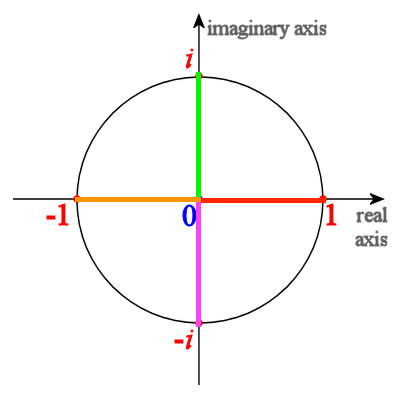
\includegraphics[width=0.5\linewidth]{plane.jpeg}
\end{center}

\subsection{Fractal for the Fourth Roots of Unity}

\begin{center}
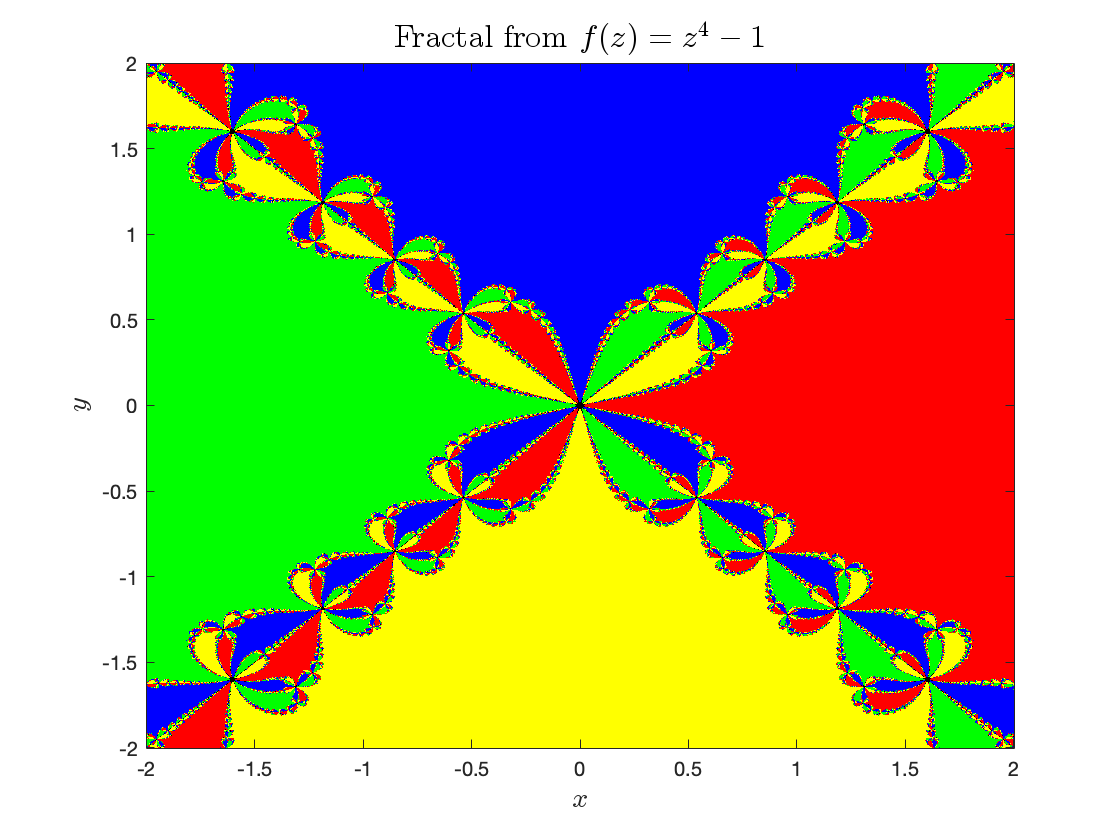
\includegraphics[width=0.7\linewidth]{z4.png}
\end{center}

\lstinputlisting{z4.m}

\subsection{Mandelbrot Fractal}

Using a similar approach, we demonstrate the Mandelbrot fractal, a fractal generated using the iteration of $f_c(z) = z^2 + c$.

\begin{center}
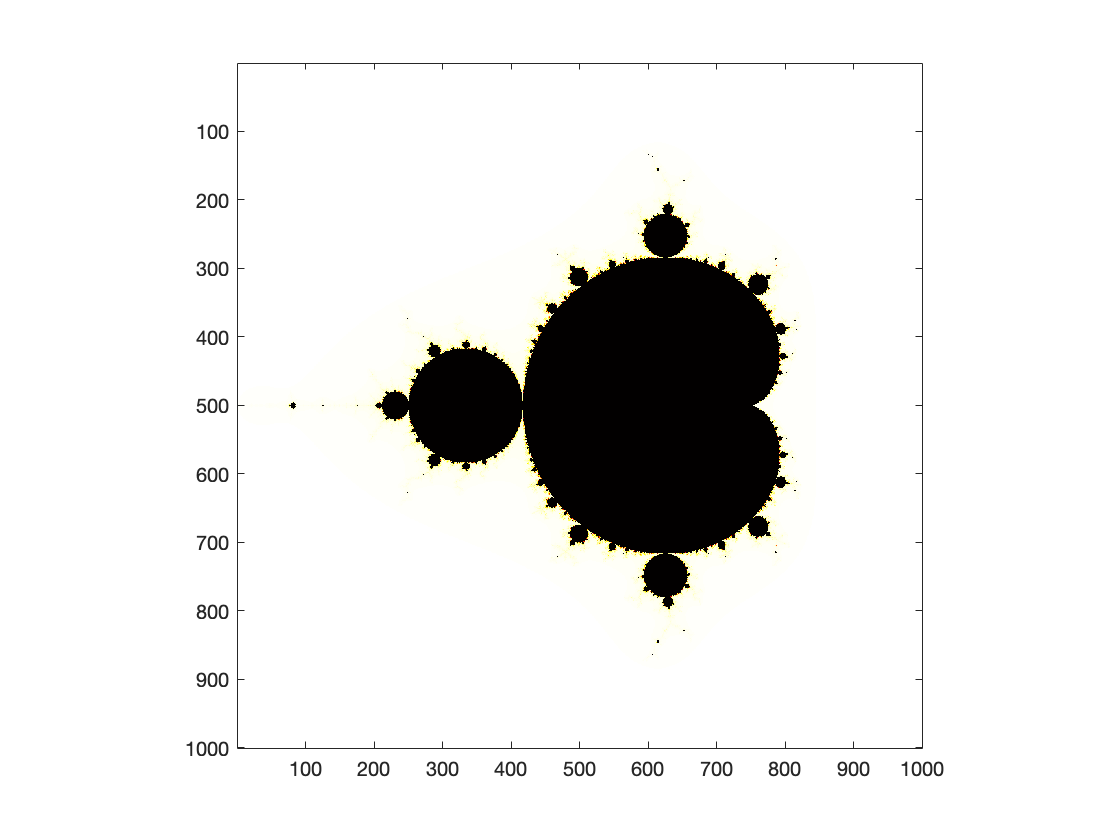
\includegraphics[width=0.7\linewidth]{mandelbrot.png}
\end{center}

\section{Summary}
\subsection{Results}
In conclusion, our exploration of Newton's method has covered its application to both simple roots and roots of multiple multiplicity. We delved into methods for determining the order of convergence and outlined approaches to approximate the order when dealing with functions whose roots are unknown. Recognizing the distinct convergence behavior for roots of multiple multiplicity, we introduced a modified version of Newton's method tailored to accelerate convergence up to the anticipated quadratic speed for roots with a multiplicity $m > 1$.

In the final sections, we showcased the broader applications of Newton's method, extending beyond root finding to the realm of fractals. Specifically, we demonstrated how Newton's method can be harnessed to generate fractals, illustrating its significance in both mathematical exploration and visualization. 

\subsection{Team Description}

Our team encountered problems with the convergence of Newton's method: we did not initially set a tolerance for when to halt the iteration. Thus, Newton's method would run for much longer than needed, attempting to find the exact value of the root. While we initially believed it was due to bad performance of the code, our profiling revealed that we were iterating much more than needed. Adding tolerance to the function let us specify the desired precision of the iteration method.

\subsection{Future Explorations}

Our team would like to further explore different fractals that can be generated using Newton's method. It would be interesting to see fractals of not just polynomial functions, but also of transcendental functions. We would like to see if there are any discernible differneces between the fractal images of functions according to their properties, such as if they are analytic, holomorphic, etc.

\subsection{References}

\begin{enumerate}

  \item Press, W. H.; Teukolsky, S. A.; Vetterling, W. T.; Flannery, B. P. (2007). \textit{Numerical Recipes: The Art of Scientific Computing (3rd ed.)}. New York: Cambridge University Press. ISBN 978-0-521-88068-8.
  
  \item Atkinson, Kendall E. (1989). \textit{An Introduction to Numerical Analysis}. John Wiley \& Sons, Inc. ISBN 0-471-62489-6.
  
  \item Press, W. H.; Teukolsky, S. A.; Vetterling, W. T.; Flannery, B. P. (2007). \textit{Numerical Recipes: The Art of Scientific Computing (3rd ed.)}. New York: Cambridge University Press. ISBN 978-0-521-88068-8. See especially Sections 9.4, 9.6, and 9.7.
  
  \item Blinn, Jim (July 1997). "Floating Point Tricks". \textit{IEEE Computer Graphics \& Applications}. 17 (4): 80. doi:10.1109/38.595279.
  
  \item Eberly, David (2001). \textit{3D Game Engine Design}. Morgan Kaufmann. ISBN 978-1-55860-593-0.
\end{enumerate}
\newpage

\section*{Appendix}

% \begin{figure}[h!]
% \centering
% \lstinputlisting{mynewton.m}
% \caption{mynewton.m}
% \label{fig:mynewton.m}
% \end{figure}

% \begin{figure}[h!]
% \centering
% \lstinputlisting{test_mynewton.m}
% \caption{test\_mynewton.m}
% \label{fig:test_mynewton.m}
% \end{figure}

\begin{figure}[h!]
  \centering
  \lstinputlisting{newtontest.m}
  \caption{newtontest.m}
  \label{fig:newtontest.m}
  \end{figure}

\begin{figure}[h!]
  \centering
  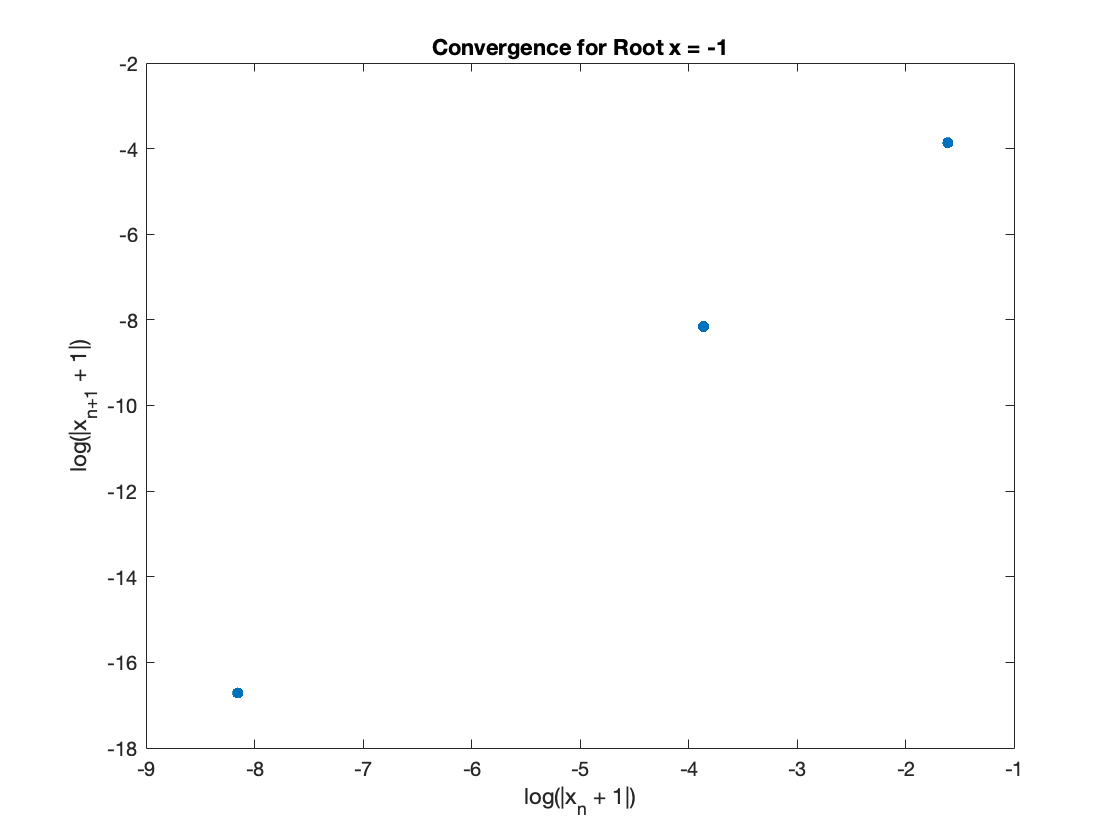
\includegraphics[width=0.8\linewidth]{newton_root_1.png}
  \caption{Log errors for $x = -1$}
  \label{fig:newton_root_1}
\end{figure}

\begin{figure}[h!]
  \centering
  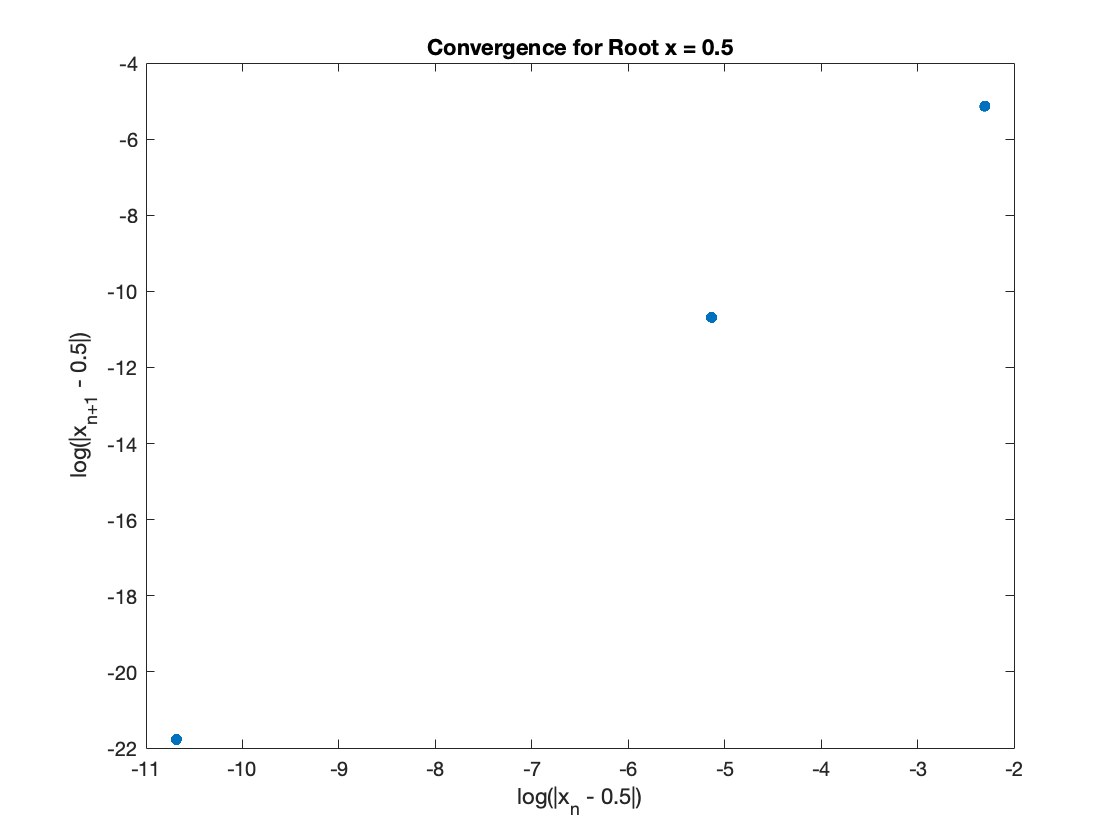
\includegraphics[width=0.8\linewidth]{newton_root_2.png}
  \caption{Log errors for $x = 1/2$}
  \label{fig:newton_root_2}
\end{figure}

\begin{figure}[h!]
  \centering
  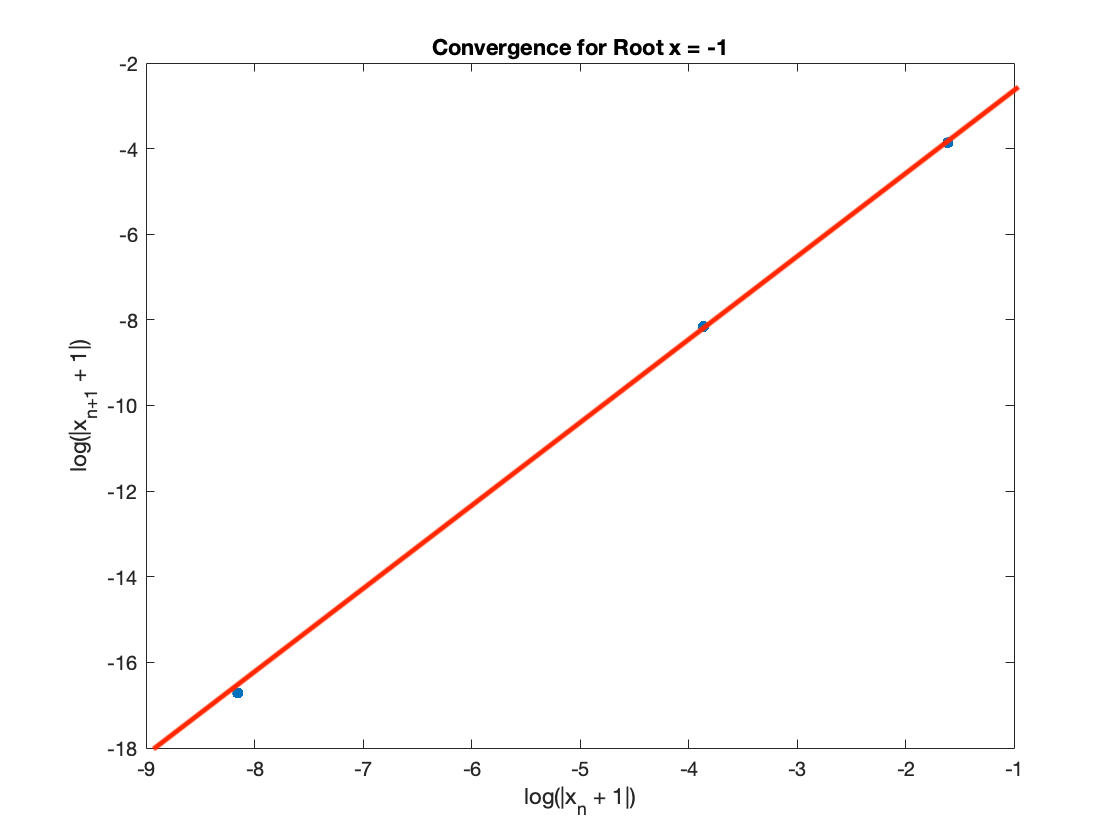
\includegraphics[width=0.8\linewidth]{newton_root_1_fit.png}
  \caption{Log errors for $x = -1$}
  \label{fig:newton_root_1_fit}
\end{figure}

\begin{figure}[h!]
  \centering
  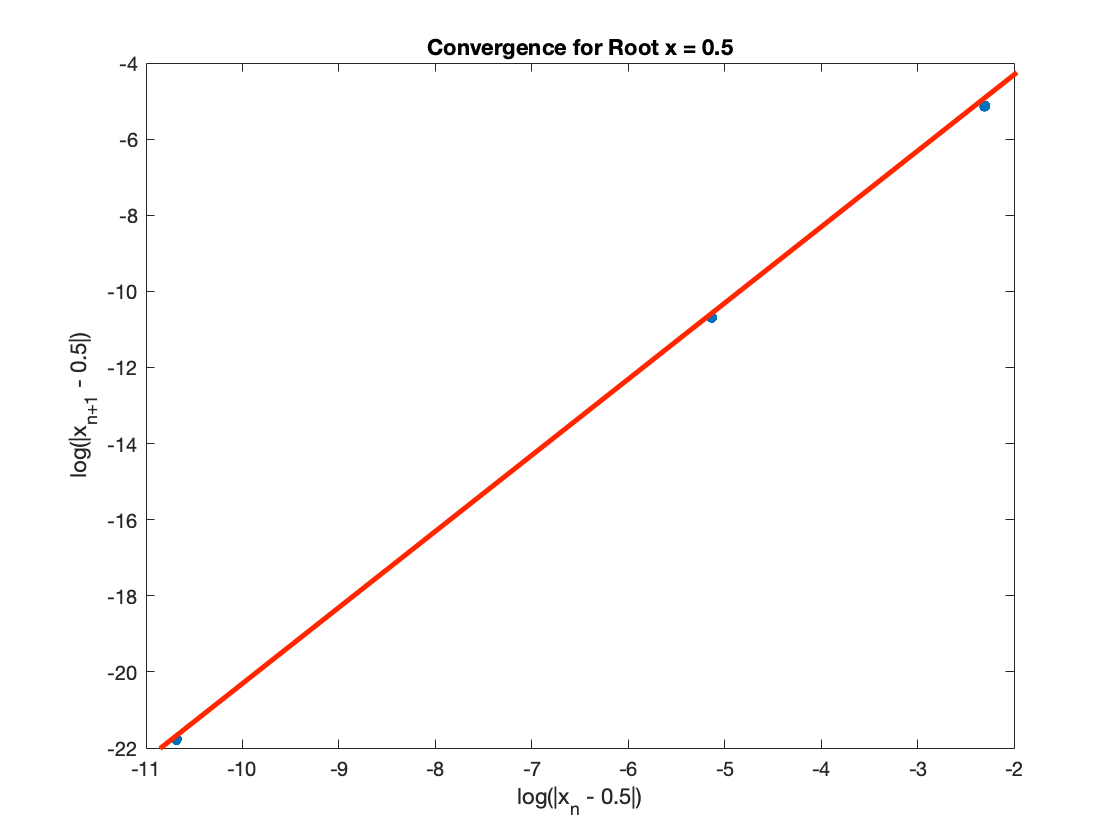
\includegraphics[width=0.8\linewidth]{newton_root_2_fit.png}
  \caption{Log errors for $x = 1/2$}
  \label{fig:newton_root_2_fit}
\end{figure}


\begin{figure}[h!]
  \centering
  \lstinputlisting{estimate_convergence.m}
  \caption{estimate\_convergence.m}
  \label{fig:estimateconvergence.m}
\end{figure}
  
\begin{figure}[h!]
  \centering
  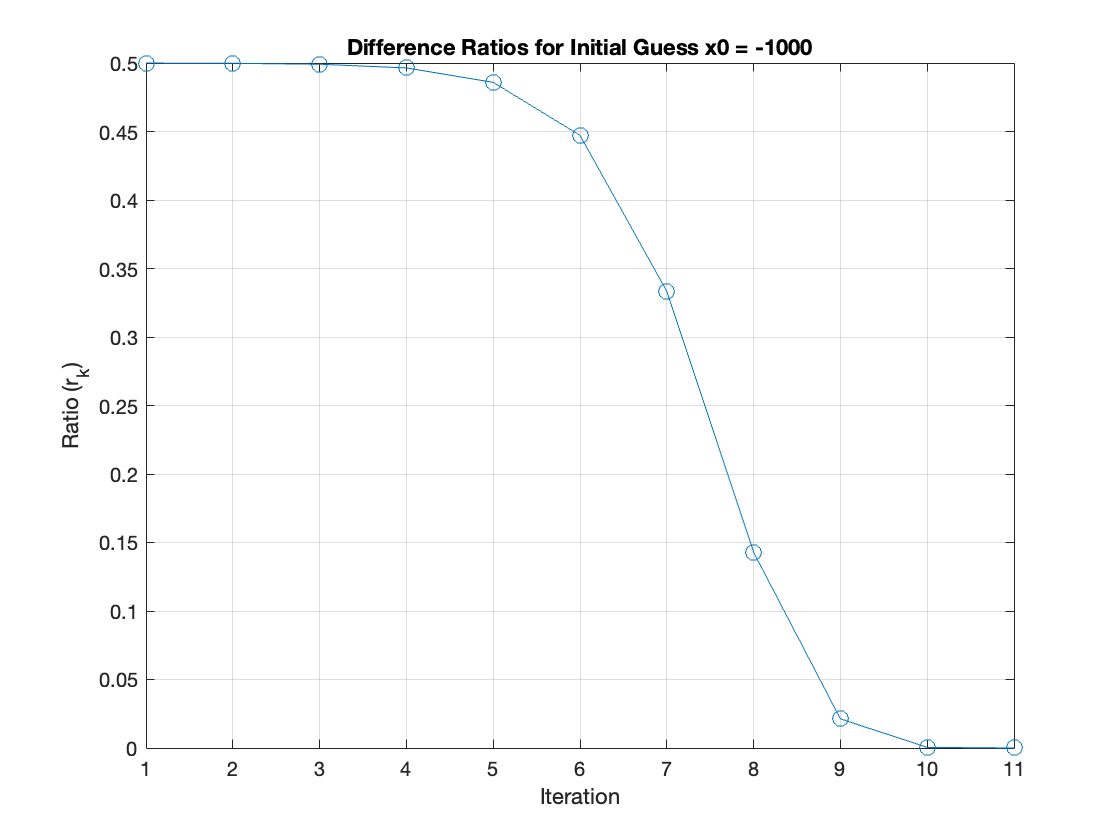
\includegraphics[width=0.8\linewidth]{estimate_convergence.png}
  \caption{Difference Ratios for an Initial Guess $x_0 = -1000$}
  \label{fig:estimate_convergence}
\end{figure}

\begin{figure}[h!]
  \centering
  \lstinputlisting{modifiednewton.m}
  \caption{modifiednewton.m}
  \label{fig:modifiednewton}
\end{figure}

% \begin{figure}[h!]
%   \centering
%   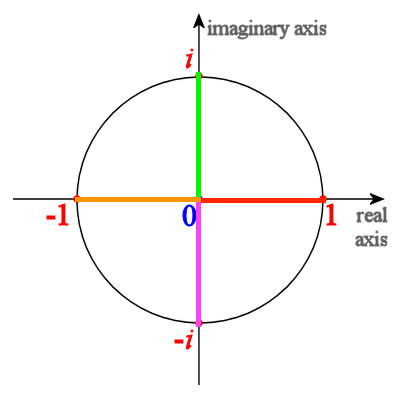
\includegraphics[width=0.8\linewidth]{plane.jpeg}
%   \caption{Complex Plane for Solutions to $z^4 = 1$}
%   \label{fig:plane}
% \end{figure}


\end{document}
